%=======================02-713 LaTeX template, following the 15-210 template==================
%
% You don't need to use LaTeX or this template, but you must turn your homework in as
% a typeset PDF somehow.
%
% How to use:
%    1. Update your information in section "A" below
%    2. Write your answers in section "B" below. Precede answers for all 
%       parts of a question with the command "\question{n}{desc}" where n is
%       the question number and "desc" is a short, one-line description of 
%       the problem. There is no need to restate the problem.
%    3. If a question has multiple parts, precede the answer to part x with the
%       command "\part{x}".
%    4. If a problem asks you to design an algorithm, use the commands
%       \algorithm, \correctness, \runtime to precede your discussion of the 
%       description of the algorithm, its correctness, and its running time, respectively.
%    5. You can include graphics by using the command \includegraphics{FILENAME}
%
\documentclass[11pt]{article}
\usepackage{amsmath,amssymb,amsthm}
\usepackage{graphicx}
\usepackage[margin=1in]{geometry}
\usepackage{fancyhdr}
\usepackage{subcaption}

\setlength{\parindent}{0pt}
\setlength{\parskip}{5pt plus 1pt}
\setlength{\headheight}{13.6pt}
\newcommand\question[2]{\vspace{.25in}\hrule\textbf{#1: #2}\vspace{.5em}\hrule\vspace{.10in}}
\renewcommand\part[1]{\vspace{.10in}\textbf{(#1)}}
\newcommand\one{\vspace{.10in}\textbf{Data1: }}
\newcommand\two{\vspace{.10in}\textbf{Data2: }}
\newcommand\three{\vspace{.10in}\textbf{Data3: }}
\pagestyle{fancyplain}
\lhead{\textbf{\NAME\ (\ANDREWID)}}
\chead{\textbf{ASS\HWNUM}}
\rhead{\today}
\begin{document}\raggedright
%Section A==============Change the values below to match your information==================
\newcommand\NAME{Yao Xiao}  % your name
\newcommand\ANDREWID{2019180015}     % your andrew id
\newcommand\HWNUM{1}              % the homework number
%Section B==============Put your answers to the questions below here=======================

% no need to restate the problem --- the graders know which problem is which,
% but replacing "The First Problem" with a short phrase will help you remember
% which problem this is when you read over your homeworks to study.

\question{1}{The First Problem} 

\part{a} \one\\
For the intertwined two spiral, using the standard bp algorithm can solve the problem very well.
In addition, the data set is not large and the data structure is not complicated. Therefore, the main adjustment directions are $learn_rate$ and epoch times. On the contrary, excessive adjustment of the hidden layer structure will be counterproductive.\\
Here is my progress report of data1:\\

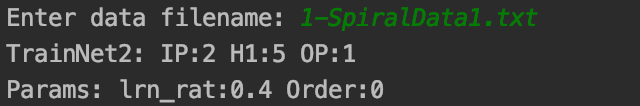
\includegraphics[scale=1]{1-in1.png}
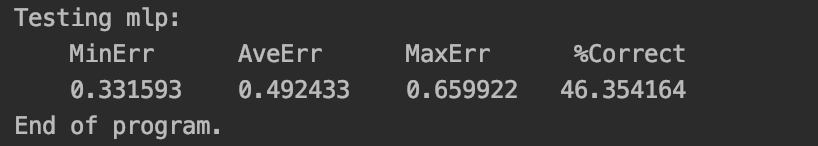
\includegraphics[scale=0.8]{1-ot1.png}
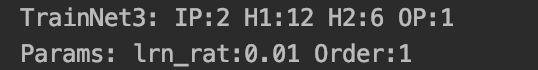
\includegraphics[scale=1]{1-in2.png}
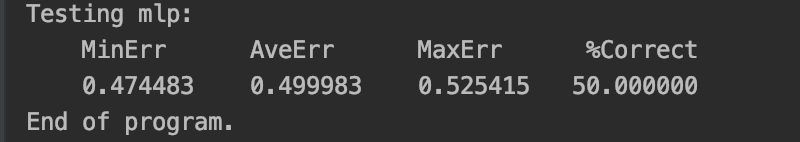
\includegraphics[scale=0.8]{1-ot2.png}
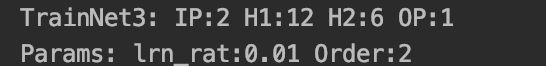
\includegraphics[scale=1]{1-in3.png}
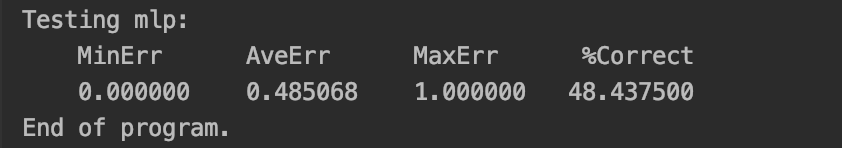
\includegraphics[scale=0.8]{1-ot3.png}
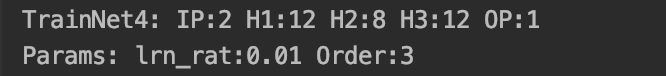
\includegraphics[scale=1]{1-in4.png}
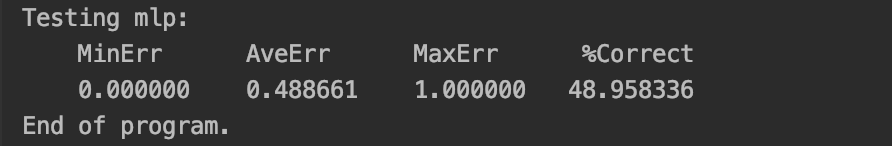
\includegraphics[scale=0.8]{1-ot4.png}

It is obvious that using a single layer neural network and setting $learn_{rate}$ to 0.4 can achieve the best experimental results.

\part{b} \two\\
For the abalone age problem, it has more features.So It may be a better way to combine the wrong samples with order3 and multi-layer neural network. Different models may have different performance, but multi-layer neural network should achieve good results.\\
Here is my progress report of data2:\\

\includegraphics[scale=1]{2-in1.png}
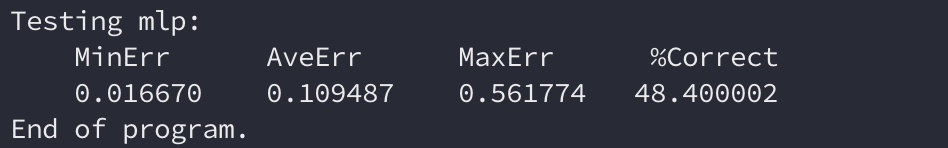
\includegraphics[scale=0.8]{2-ot1.png}
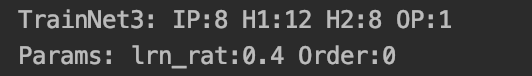
\includegraphics[scale=1]{2-in2.png}
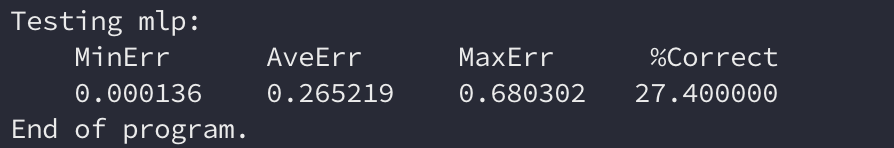
\includegraphics[scale=0.8]{2-ot2.png}

\includegraphics[scale=1]{2-in3.png}
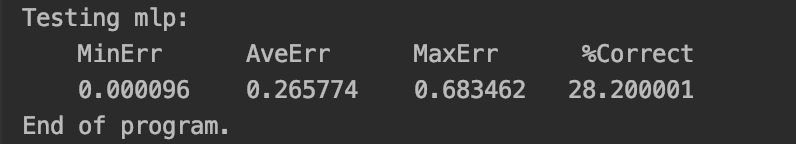
\includegraphics[scale=0.8]{2-ot3.png}

It can be seen that Order3 with a three-layer structure and Order0 with a two-layer structure have achieved good results. The advantages and disadvantages of the two need to be further explored.

\part{c} \three\\
For the SPECT Heart Diagnosis problem, considering that it has very input values, too many neural networks may affect the calculation, so try to adjust the rate and single layer structure.\\
Here is my progress report of data3:\\
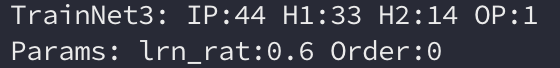
\includegraphics[scale=1]{3-in1.png}
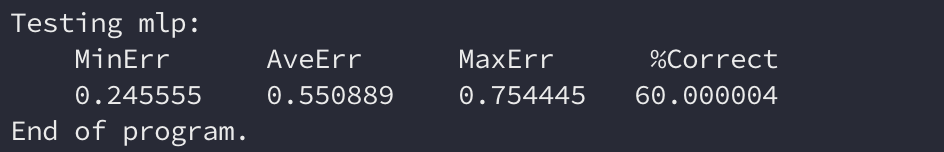
\includegraphics[scale=0.8]{3-ot1.png}
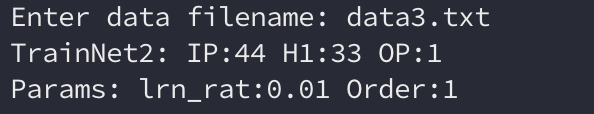
\includegraphics[scale=1]{3-in2.png}
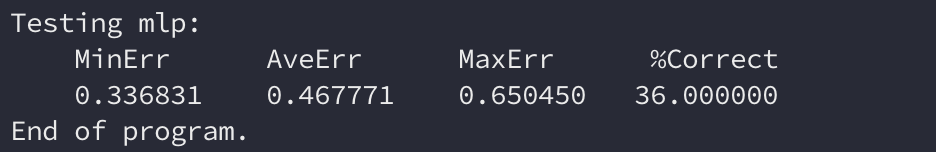
\includegraphics[scale=0.8]{3-ot2.png}

It can be seen that a single-layer neural network achieves better results than a multi-layer.


\question{2}{The Second Problem}

\part{a} \one\\
To be able to learn classification correctly the experiment shows that the mlp that is most suitable for problem 1 is a structure of 5 neurons in a single layer, and the learning rate is 0.4 and a suitable number of iterations is 10000 at the same time, each setting can see in Figure 1:\\

\begin{figure}[!ht]
    \centering
    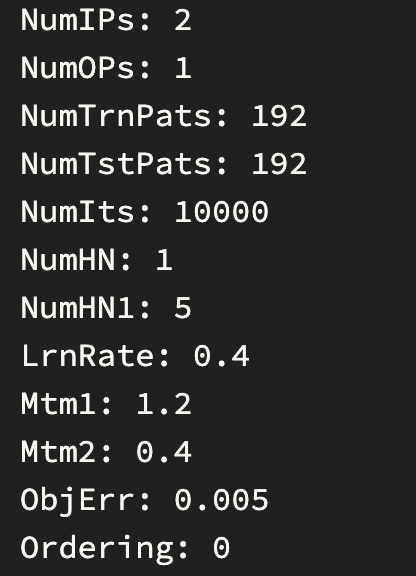
\includegraphics[scale=0.8]{1-par.png}
    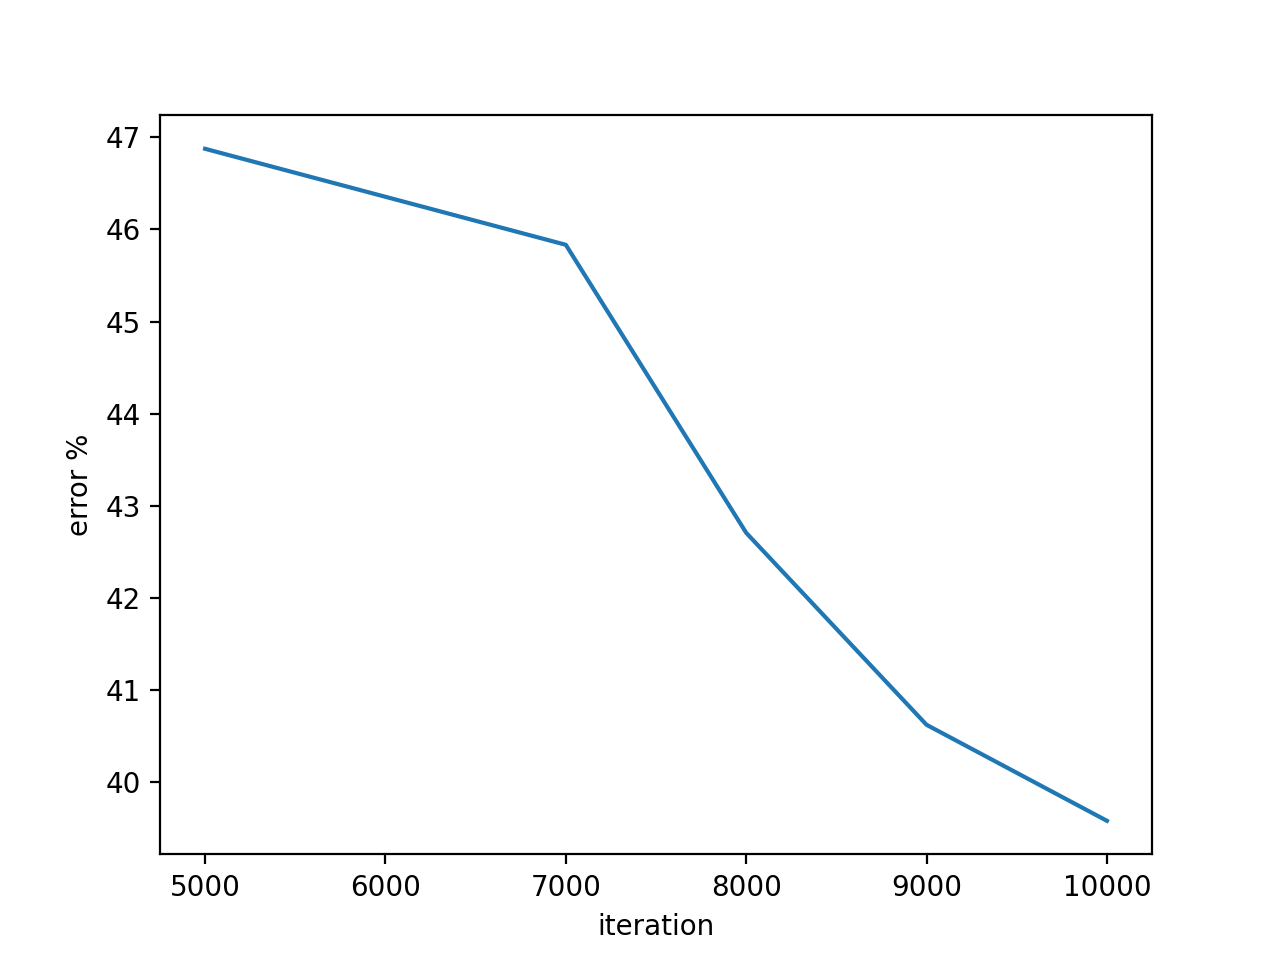
\includegraphics[scale=1]{Figure_1.png}
    \caption{d1 parameters and error vs iteration}
\end{figure}


\part{b} \two\\
To be able to learn classification correctly, by comparison, the mlp that is most suitable for problem 2 is a two-layer neural network with nodes 12 and 8, and a suitable number of iterations is 8000, each set can see in Figure 2 adn Figure 3:
\begin{figure}[!ht]
    \centering
    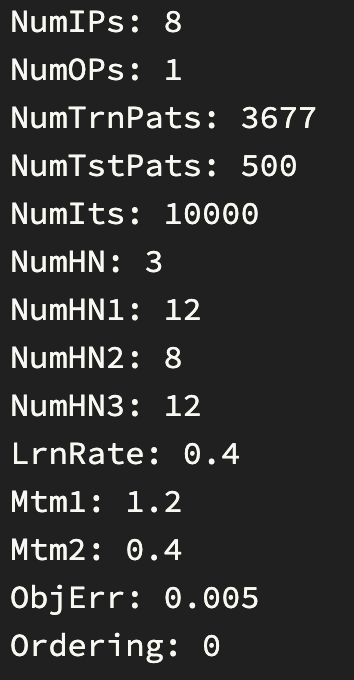
\includegraphics[scale=0.8]{2-2par.png}
    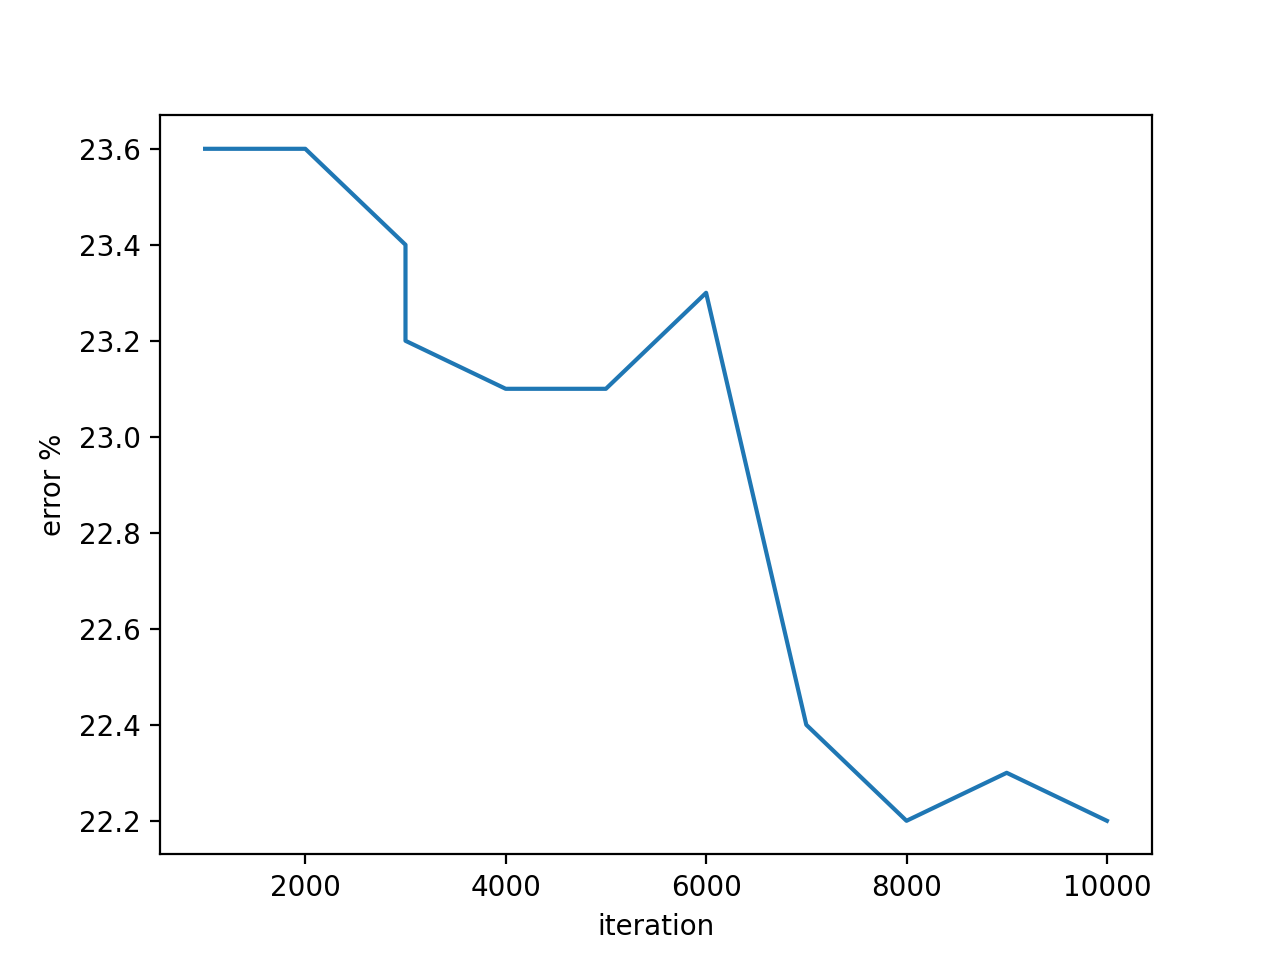
\includegraphics[scale=1]{Figure_2-2.png}
	\caption{d2.1 parameters and error vs iteration}
\end{figure}

\begin{figure}[!ht]
    \centering
    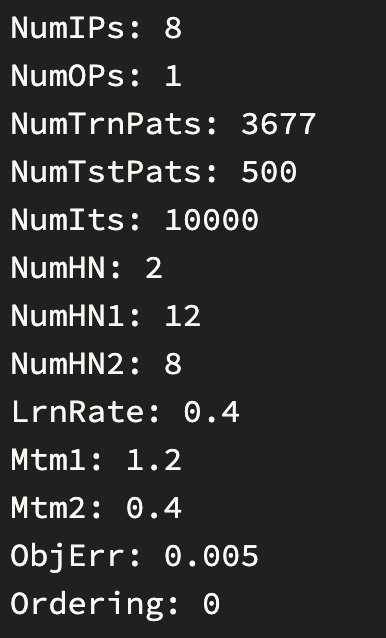
\includegraphics[scale=0.8]{2-1par.png}
    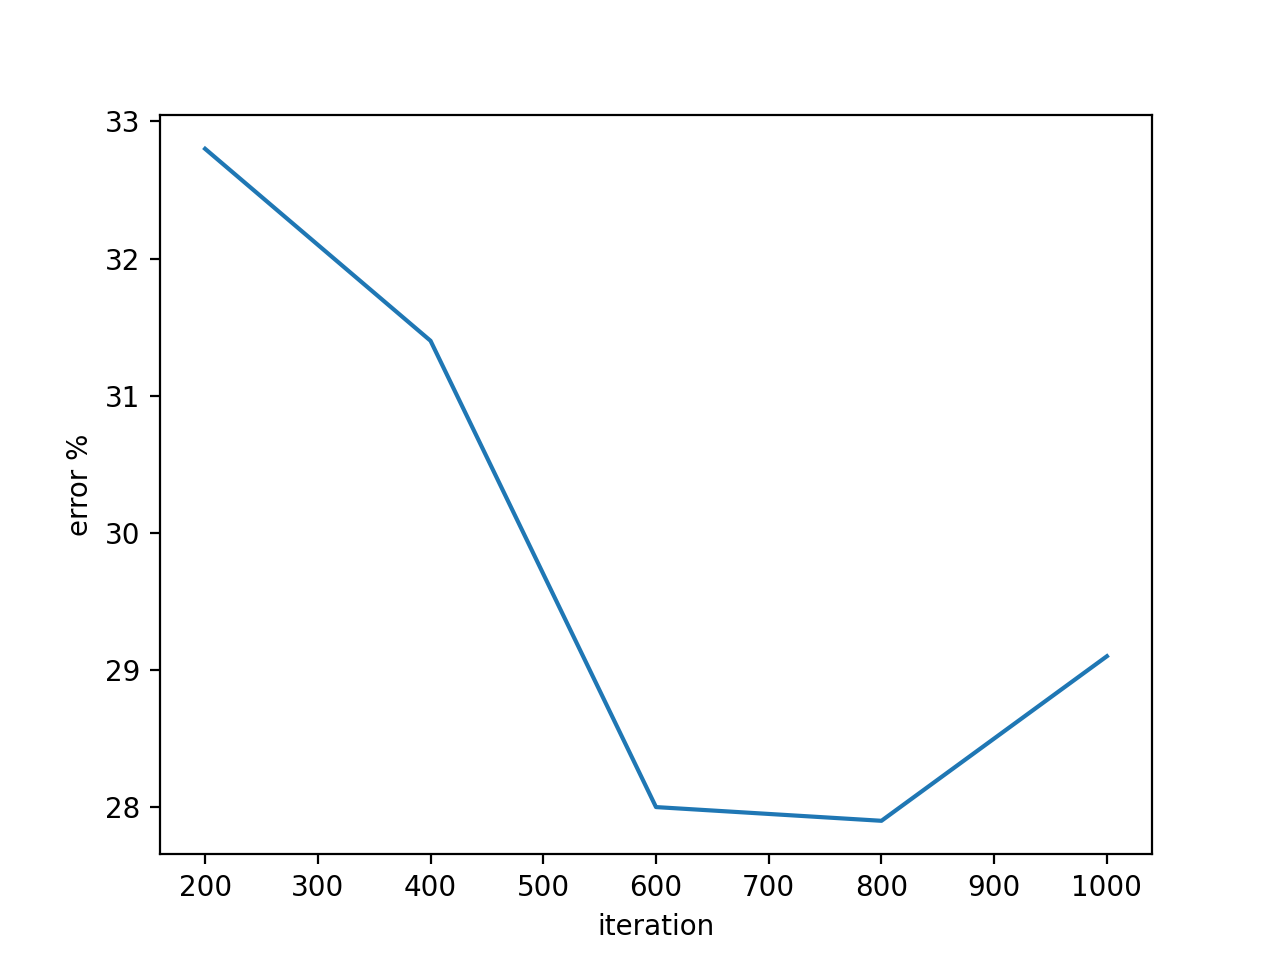
\includegraphics[scale=1]{Figure_2-1.png}
	\caption{d2.2 parameters and error vs iteration}
\end{figure}


\part{c} \three\\
To be able to learn classification correctly, the experiment shows that the MLP that is most suitable for Problem 3 is a single-layer hidden layer but contains a large number of nodes. The appropriate number of iterations is 6000, and each setting can see in Figure 4:\\
\begin{figure}[!ht]
    \centering
    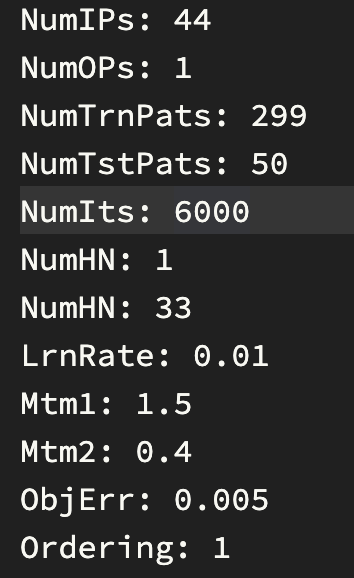
\includegraphics[scale=0.8]{3-par.png}
    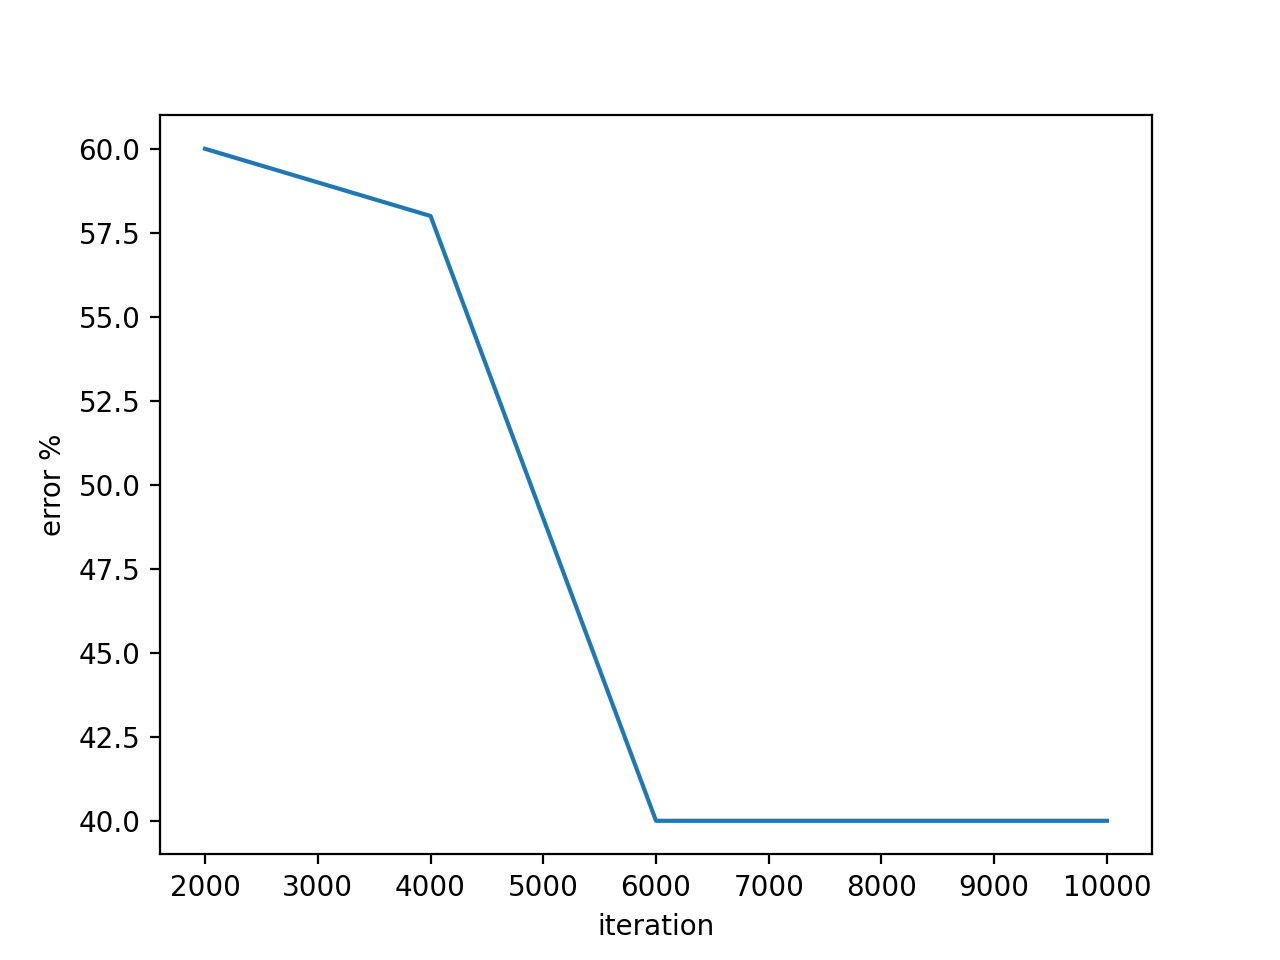
\includegraphics[scale=1]{Figure_3.png}
	\caption{d3 parameters and error vs iteration}
\end{figure}


\end{document}
